%%
%% Automatically generated file from DocOnce source
%% (https://github.com/hplgit/doconce/)
%%
%%
% #ifdef PTEX2TEX_EXPLANATION
%%
%% The file follows the ptex2tex extended LaTeX format, see
%% ptex2tex: http://code.google.com/p/ptex2tex/
%%
%% Run
%%      ptex2tex myfile
%% or
%%      doconce ptex2tex myfile
%%
%% to turn myfile.p.tex into an ordinary LaTeX file myfile.tex.
%% (The ptex2tex program: http://code.google.com/p/ptex2tex)
%% Many preprocess options can be added to ptex2tex or doconce ptex2tex
%%
%%      ptex2tex -DMINTED myfile
%%      doconce ptex2tex myfile envir=minted
%%
%% ptex2tex will typeset code environments according to a global or local
%% .ptex2tex.cfg configure file. doconce ptex2tex will typeset code
%% according to options on the command line (just type doconce ptex2tex to
%% see examples). If doconce ptex2tex has envir=minted, it enables the
%% minted style without needing -DMINTED.
% #endif

% #define PREAMBLE

% #ifdef PREAMBLE
%-------------------- begin preamble ----------------------

\documentclass[%
oneside,                 % oneside: electronic viewing, twoside: printing
final,                   % draft: marks overfull hboxes, figures with paths
10pt]{article}

\listfiles               %  print all files needed to compile this document

\usepackage{relsize,makeidx,color,setspace,amsmath,amsfonts,amssymb}
\usepackage[table]{xcolor}
\usepackage{bm,ltablex,microtype}

\usepackage[pdftex]{graphicx}

\usepackage{ptex2tex}
% #ifdef MINTED
\usepackage{minted}
\usemintedstyle{default}
% #endif
\usepackage{fancyvrb}

\usepackage[T1]{fontenc}
%\usepackage[latin1]{inputenc}
\usepackage{ucs}
\usepackage[utf8x]{inputenc}

\usepackage{lmodern}         % Latin Modern fonts derived from Computer Modern

% Hyperlinks in PDF:
\definecolor{linkcolor}{rgb}{0,0,0.4}
\usepackage{hyperref}
\hypersetup{
    breaklinks=true,
    colorlinks=true,
    linkcolor=linkcolor,
    urlcolor=linkcolor,
    citecolor=black,
    filecolor=black,
    %filecolor=blue,
    pdfmenubar=true,
    pdftoolbar=true,
    bookmarksdepth=3   % Uncomment (and tweak) for PDF bookmarks with more levels than the TOC
    }
%\hyperbaseurl{}   % hyperlinks are relative to this root

\setcounter{tocdepth}{2}  % levels in table of contents

% Tricks for having figures close to where they are defined:
% 1. define less restrictive rules for where to put figures
\setcounter{topnumber}{2}
\setcounter{bottomnumber}{2}
\setcounter{totalnumber}{4}
\renewcommand{\topfraction}{0.95}
\renewcommand{\bottomfraction}{0.95}
\renewcommand{\textfraction}{0}
\renewcommand{\floatpagefraction}{0.75}
% floatpagefraction must always be less than topfraction!
% 2. ensure all figures are flushed before next section
\usepackage[section]{placeins}
% 3. enable begin{figure}[H] (often leads to ugly pagebreaks)
%\usepackage{float}\restylefloat{figure}

% --- fancyhdr package for fancy headers ---
\usepackage{fancyhdr}
\fancyhf{} % sets both header and footer to nothing
\renewcommand{\headrulewidth}{0pt}
\fancyfoot[LE,RO]{\thepage}
% Ensure copyright on titlepage (article style) and chapter pages (book style)
\fancypagestyle{plain}{
  \fancyhf{}
  \fancyfoot[C]{{\footnotesize \copyright\ 2023, UP Mathématiques. ESPRIT}}
%  \renewcommand{\footrulewidth}{0mm}
  \renewcommand{\headrulewidth}{0mm}
}
% Ensure copyright on titlepages with \thispagestyle{empty}
\fancypagestyle{empty}{
  \fancyhf{}
  \fancyfoot[C]{{\footnotesize \copyright\ 2023, UP Mathématiques. ESPRIT}}
  \renewcommand{\footrulewidth}{0mm}
  \renewcommand{\headrulewidth}{0mm}
}

\pagestyle{fancy}


\usepackage[framemethod=TikZ]{mdframed}

% --- begin definitions of admonition environments ---

% Admonition style "mdfbox" is an oval colored box based on mdframed
% "notice" admon
\colorlet{mdfbox_notice_background}{gray!5}
\newmdenv[
  skipabove=15pt,
  skipbelow=15pt,
  outerlinewidth=0,
  backgroundcolor=mdfbox_notice_background,
  linecolor=black,
  linewidth=2pt,       % frame thickness
  frametitlebackgroundcolor=mdfbox_notice_background,
  frametitlerule=true,
  frametitlefont=\normalfont\bfseries,
  shadow=false,        % frame shadow?
  shadowsize=11pt,
  leftmargin=0,
  rightmargin=0,
  roundcorner=5,
  needspace=0pt,
]{notice_mdfboxmdframed}

\newenvironment{notice_mdfboxadmon}[1][]{
\begin{notice_mdfboxmdframed}[frametitle=#1]
}
{
\end{notice_mdfboxmdframed}
}

% Admonition style "mdfbox" is an oval colored box based on mdframed
% "summary" admon
\colorlet{mdfbox_summary_background}{gray!5}
\newmdenv[
  skipabove=15pt,
  skipbelow=15pt,
  outerlinewidth=0,
  backgroundcolor=mdfbox_summary_background,
  linecolor=black,
  linewidth=2pt,       % frame thickness
  frametitlebackgroundcolor=mdfbox_summary_background,
  frametitlerule=true,
  frametitlefont=\normalfont\bfseries,
  shadow=false,        % frame shadow?
  shadowsize=11pt,
  leftmargin=0,
  rightmargin=0,
  roundcorner=5,
  needspace=0pt,
]{summary_mdfboxmdframed}

\newenvironment{summary_mdfboxadmon}[1][]{
\begin{summary_mdfboxmdframed}[frametitle=#1]
}
{
\end{summary_mdfboxmdframed}
}

% Admonition style "mdfbox" is an oval colored box based on mdframed
% "warning" admon
\colorlet{mdfbox_warning_background}{gray!5}
\newmdenv[
  skipabove=15pt,
  skipbelow=15pt,
  outerlinewidth=0,
  backgroundcolor=mdfbox_warning_background,
  linecolor=black,
  linewidth=2pt,       % frame thickness
  frametitlebackgroundcolor=mdfbox_warning_background,
  frametitlerule=true,
  frametitlefont=\normalfont\bfseries,
  shadow=false,        % frame shadow?
  shadowsize=11pt,
  leftmargin=0,
  rightmargin=0,
  roundcorner=5,
  needspace=0pt,
]{warning_mdfboxmdframed}

\newenvironment{warning_mdfboxadmon}[1][]{
\begin{warning_mdfboxmdframed}[frametitle=#1]
}
{
\end{warning_mdfboxmdframed}
}

% Admonition style "mdfbox" is an oval colored box based on mdframed
% "question" admon
\colorlet{mdfbox_question_background}{gray!5}
\newmdenv[
  skipabove=15pt,
  skipbelow=15pt,
  outerlinewidth=0,
  backgroundcolor=mdfbox_question_background,
  linecolor=black,
  linewidth=2pt,       % frame thickness
  frametitlebackgroundcolor=mdfbox_question_background,
  frametitlerule=true,
  frametitlefont=\normalfont\bfseries,
  shadow=false,        % frame shadow?
  shadowsize=11pt,
  leftmargin=0,
  rightmargin=0,
  roundcorner=5,
  needspace=0pt,
]{question_mdfboxmdframed}

\newenvironment{question_mdfboxadmon}[1][]{
\begin{question_mdfboxmdframed}[frametitle=#1]
}
{
\end{question_mdfboxmdframed}
}

% Admonition style "mdfbox" is an oval colored box based on mdframed
% "block" admon
\colorlet{mdfbox_block_background}{gray!5}
\newmdenv[
  skipabove=15pt,
  skipbelow=15pt,
  outerlinewidth=0,
  backgroundcolor=mdfbox_block_background,
  linecolor=black,
  linewidth=2pt,       % frame thickness
  frametitlebackgroundcolor=mdfbox_block_background,
  frametitlerule=true,
  frametitlefont=\normalfont\bfseries,
  shadow=false,        % frame shadow?
  shadowsize=11pt,
  leftmargin=0,
  rightmargin=0,
  roundcorner=5,
  needspace=0pt,
]{block_mdfboxmdframed}

\newenvironment{block_mdfboxadmon}[1][]{
\begin{block_mdfboxmdframed}[frametitle=#1]
}
{
\end{block_mdfboxmdframed}
}

% --- end of definitions of admonition environments ---

% prevent orhpans and widows
\clubpenalty = 10000
\widowpenalty = 10000

% --- end of standard preamble for documents ---


% insert custom LaTeX commands...

\raggedbottom
\makeindex

%-------------------- end preamble ----------------------

\begin{document}

% matching end for #ifdef PREAMBLE
% #endif

\newcommand{\exercisesection}[1]{\subsection*{#1}}


% ------------------- main content ----------------------



% ----------------- title -------------------------

\title{Introduction à Python (I)}

% ----------------- author(s) -------------------------

\author{UP Mathématiques\inst{1}}
\institute{École Supérieure PRivée d'Ingénierie et de Technologies.\inst{1}}
% ----------------- end author(s) -------------------------

\date{2 novembre 2023
% <optional titlepage figure>
% <optional copyright>
}

% !split
\section{Objectifs généraux en premier}

Une partie essentielle de ce cours est de vous permettre de faire de la science par des expériences numériques et de développer des projets qui vous permettent d'étudier des systèmes complexes. Le but est d'améliorer ce que nous appelons la pensée algorithmique.

\paragraph{Algorithme}
Un ensemble fini d'instructions non ambiguës qui, étant donné un ensemble de conditions initiales, peuvent être effectuées dans une séquence prescrite pour atteindre un certain but.

% !split
\section{Situation standard que nous rencontrons quotidiennement}

La situation standard que nous rencontrons presque tous les séances de cours:

\begin{itemize}
\item Théorie + expérience + simulation est presque la norme dans la recherche et l'industrie.

\item Être capable de modéliser des systèmes complexes. Résoudre de vrais problèmes.

\item Accent la compréhension des principes fondamentaux et des lois dans les sciences.

\item Être capable de visualiser, présenter, discuter, interpréter et venir avec une analyse critique des résultats, et développer une attitude éthique saine pour son propre travail.

\item Améliorer le raisonnement sur la méthode scientifique.
\end{itemize}

\noindent
Une bonne présentation des résultats obtenus via de bons rapports scientifiques, aide à inclure tous les aspects ci-dessus.

% !split
\section{Langage Python}

\href{{http://www.python.org/}}{Python} est un langage de programmation moderne de haut niveau, orienté objet et d'usage général.

\textbf{Caractéristiques générales de Python} :

\begin{itemize}
\item Langage simple:
\begin{itemize}

  \item facile à lire et à apprendre avec une syntaxe minimaliste.

\end{itemize}

\noindent
\item Langage concis et expressif:
\begin{itemize}

  \item moins de lignes de code

  \item moins de bugs

  \item plus facile à maintenir.
\end{itemize}

\noindent
\end{itemize}

\noindent
% !split
\textbf{Détails techniques} :

\begin{itemize}
\item Typé dynamiquement:
\begin{itemize}

  \item Pas besoin de définir le type des variables, les arguments ou le type des fonctions.

\end{itemize}

\noindent
\item La gestion automatique de la mémoire:
\begin{itemize}

  \item Aucune nécessité d'allouer explicitement et désallouer la mémoire pour les variables et les tableaux de données. Aucun bug de fuite de mémoire.

\end{itemize}

\noindent
\item Interprété:
\begin{itemize}

  \item Pas besoin de compiler le code. L'interpréteur Python lit et exécute le code python directement.
\end{itemize}

\noindent
\end{itemize}

\noindent
% !split
\textbf{Avantages} :

\begin{itemize}
\item Le principal avantage est la facilité de programmation, qui minimise le temps nécessaire pour développer, déboguer et maintenir le code.

\item Langage bien conçu qui encourage les bonnes pratiques de programmation:
\begin{itemize}

  \item Modulaire et orientée objet, permet l'encapsulation  et la réutilisation de code. Il en résulte souvent un code plus transparent, plus facile à améliorer et sans bug.

  \item Documentation intégré avec le code.

\end{itemize}

\noindent
\item De nombreuses bibliothèques standards, et de nombreux packages add-on.
\end{itemize}

\noindent
% !split
\section{Installation d'un environnement Python scientifique}

\subsection{Installation sur ordinateur}

\paragraph{Qu’est ce que Anaconda ?}
L’installation d’un environnement Python complet peut-être une vraie galère. Déjà, il faut télécharger Python et l’installer. Par la suite, télécharger un à un les packages dont on a besoin. Parfois, le nombre de ces librairies peut-être grand.

Par ailleurs, il faut s’assurer de la compatibilité entre les versions des différentes packages qu’on a à télécharger. Bref, ce n’est pas amusant.

% !split
\href{{https://www.anaconda.com/download/}}{Anaconda} est  une distribution Python. A son installation, Anaconda installera Python ainsi qu'une multitude de packages (voir \href{{https://docs.anaconda.com/anaconda/packages/pkg-docs#python-3-6}}{liste de packages anaconda}).  Cela nous évite de nous ruer dans les problèmes d’incompatibilités entre les différents packages.

Finalement, Anaconda propose un outil de gestion de packages appelé \href{{https://conda.io/docs/}}{conda}. Ce dernier permettra de mettre à jour et installer facilement les librairies dont on aura besoin pour nos développements.

% !split
\paragraph{Préparer la formation: téléchargement d’Anaconda.}
Nous demandons à tous les étudiants de télécharger Anaconda. Pour cela, il faut télécharger un installeur à partir de \href{{https://www.anaconda.com/download/}}{\nolinkurl{https://www.anaconda.com/download/}}, correspondant à votre système d’exploitation (Windows, Mac OS X, Linux). Il faut choisir entre 32 bits ou 64 bits (pour la version \emph{Python 3}) selon que votre système d’exploitation est 32 bits ou 64 bits.
% !split


\begin{figure}[!ht]  % 
  \centerline{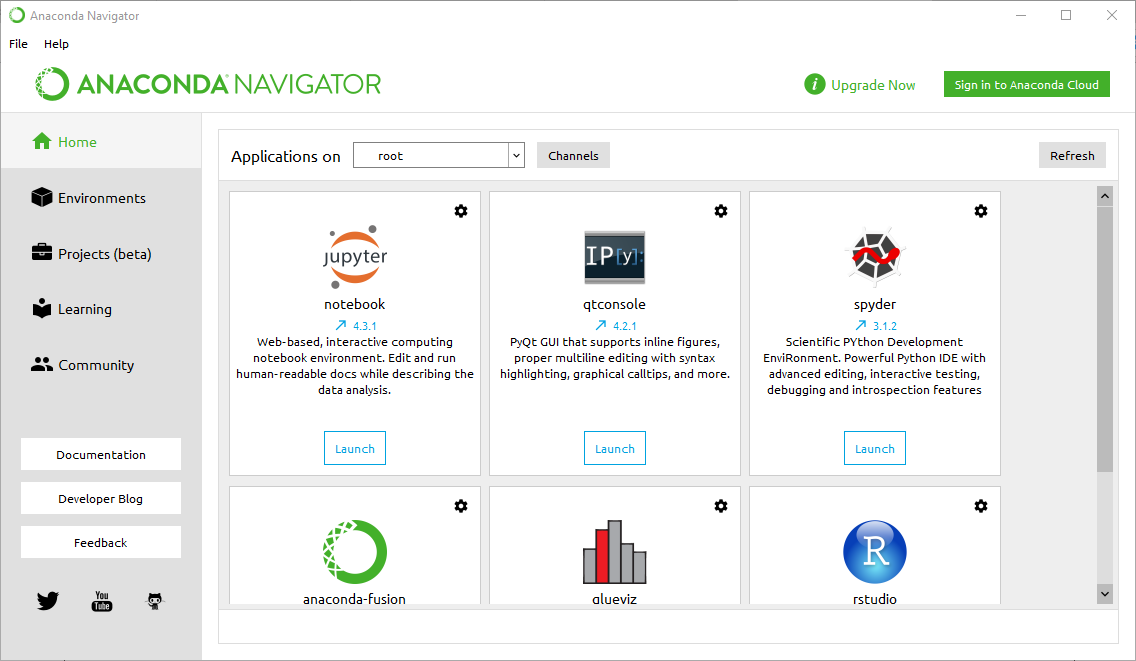
\includegraphics[width=0.7\linewidth]{imgs/AnacondaNavigator.png}}
  \caption{
  Interface graphique du navigateur Anaconda sur Windows
  }
\end{figure}
%\clearpage % flush figures 


% !split
\begin{block}{Notice}
Anaconda installe plusieurs exécutables pour développer en Python dans le répertoire \emph{anaconda/bin}, sans toujours créer des raccourcis sur le bureau ou dans un menu. Nous nous occuperons au tout début de la formation de créer des raccourcis pour pouvoir lancer l'application web \emph{Jupyter notebook}. Vous pouvez lancer le notebook depuis le navigateur Anaconda.
\end{block}

% !split
\section{Introduction: "Hello World!"}
C'est devenu une tradition que lorsque vous apprenez un nouveau langage de programmation, vous démarrez avec un programme permettant à l'ordinateur d'imprimer le message \emph{"Hello World!"}.

\bipy
In [1]: print("Hello World!")
Hello World!
\eipy

Félicitation! tout à l'heure vous avez fait votre ordinateur saluer le monde en anglais! La fonction \texttt{print()} est utilisée pour imprimer l’instruction entre les parenthèses. De plus, l'utilisation de guillemets simples \Verb?print('Hello World!')? affichera le même résultat. Le délimiteur de début et de fin doit être le même.

\bipy
In [2]: print('Hello World!')
Hello World!
\eipy

% !split
\section{Commentaires}

Au fur et à mesure que vos programmes deviennent plus grands et plus compliqués, ils deviennent plus difficiles à lire et à regarder un morceau de code et à comprendre ce qu'il fait ou pourquoi. Pour cette raison, il est conseillé d’ajouter des notes à vos programmes pour expliquer en langage naturel ce qu’il fait. Ces notes s'appellent des commentaires et commencent par le symbole \Verb!#!.

Voyez ce qui se passe lorsque nous ajoutons un commentaire au code précédent:

\bipy
In [3]: print('Hello World!') # Ceci est mon premier commentaire
Hello World!
\eipy
Rien ne change dans la sortie? Oui, et c’est très normal, l’interprète Python ignore cette ligne et ne renvoie rien. La raison en est que les commentaires sont écrits pour les humains, pour comprendre leurs codes, et non pour les machines.

% !split
\section{Nombres}

L'interpréteur Python agit comme une simple calculatrice: vous pouvez y taper une expression et l'interpréteur restituera la valeur. La syntaxe d'expression est simple: les opérateurs +, -, * et / fonctionnent comme dans la plupart des autres langages (par exemple, Pascal ou C); les parenthèses (\texttt{()}) peuvent être utilisées pour le regroupement. Par exemple:

\bipy
In [4]: 5+3
Out[4]: 8
In [5]: 2 - 9      # les espaces sont optionnels
Out[5]: -7
In [6]: 7 + 3 * 4  #la hiérarchie des opérations mathématique
Out[6]: 19
In [7]: (7 + 3) * 4  # est-elle respectées?
Out[7]: 40
# en python3 la division retourne toujours un nombre en virgule flottante
In [8]: 20 / 3
Out[8]: 6.666666666666667
In [9]: 7 // 2      # une division entière
Out[9]: 3
\eipy

% !split
On peut noter l’existence de l’opérateur \Verb!%! (appelé opérateur modulo). Cet opérateur fournit le reste de la division entière d’un nombre par un autre. Par exemple :

\bipy
In [10]: 7 % 2       # donne le reste de la division
Out[10]: 1
In [11]: 6 % 2
Out[11]: 0
\eipy

Les exposants peuvent être calculés à l'aide de doubles astérisques \texttt{**}.

\bipy
In [12]: 3**2
Out[12]: 9
\eipy

Les puissances de dix peuvent être calculées comme suit:

\bipy
In [13]: 3 * 2e3   # vaut 3 * 2000
Out[13]: 6000.0
\eipy
% !split
\section{Affectations (ou assignation)}

\subsection{variables}
Dans presque tous les programmes Python que vous allez écrire, vous aurez des variables. Les variables agissent comme des espaces réservés pour les données. Ils peuvent aider à court terme, ainsi qu’à la logique, les variables pouvant changer, d’où leur nom. C’est beaucoup plus facile en Python car aucune déclaration de variables n’est requise. Les noms de variable (ou tout autre objet Python tel que fonction, classe, module, etc.) commencent par une lettre majuscule ou minuscule (A-Z ou a-z). Ils sont sensibles à la casse (\texttt{VAR1} et \texttt{var1} sont deux variables distinctes). Depuis Python, vous pouvez utiliser n’importe quel caractère Unicode, il est préférable d’ignorer les caractères ASCII (donc pas de caractères accentués).

Si une variable est nécessaire, pensez à un nom et commencez à l'utiliser comme une variable, comme dans l'exemple ci-dessous:

% !split
Pour calculer l'aire d'un rectangle par exemple: \texttt{largeur} x \texttt{hauteur}:

\bipy
In [15]: largeur = 25
    ...: hauteur = 40
    ...: largeur    # essayer d'accéder à la valeur de la variable largeur
Out[15]: 25
\eipy

on peut également utiliser la fonction \texttt{print()} pour afficher la valeur de la variable \texttt{largeur}

\bipy
In [16]: print(largeur)
25
\eipy
Le produit de ces deux variables donne l'aire du rectangle:
\bipy
In [17]: largeur * hauteur  # donne l'aire du rectangle
Out[17]: 1000
\eipy
% !split
\begin{block}{Notice}
Notez ici que le signe égal (\texttt{=}) dans l'affectation ne doit pas être considéré comme \textbf{"est égal à"}. Il doit être \textbf{"lu"} ou interprété comme \textbf{"est définie par"}, ce qui signifie dans notre exemple:

\begin{quote}
La variable \texttt{largeur} est définie par la valeur 25 et la variable \texttt{hauteur} est définie par la valeur 40.
\end{quote}

\end{block}

\begin{block}{Warning}
Si une variable n'est pas \emph{définie} (assignée à une valeur), son utilisation vous donnera une erreur:

\bipy
In [18]: aire     # essayer d'accéder à une variable non définie
-----------------------------------------------------------------------
NameError                            Traceback (most recent call last)
<ipython-input-18-1b03529c1ce5> in <module>()
----> 1 aire     # essayer d'accéder à une variable non définie

NameError: name 'aire' is not defined
\eipy
\end{block}
% !split

Laissez-nous résoudre ce problème informatique (ou \textbf{bug} tout simplement)!. En d'autres termes, assignons la variable \texttt{aire} à sa valeur.

\bipy
In [19]: aire = largeur * hauteur
    ...: aire  # et voila!
Out[19]: 1000
\eipy

\subsection{Noms de variables réservés (keywords)}
Certains noms de variables ne sont pas disponibles, ils sont réservés à python lui-même. Les mots-clés suivants (que vous pouvez afficher dans l'interpréteur avec la commande \texttt{help("keywords")}) sont réservés et ne peuvent pas être utilisés pour définir vos propres identifiants (variables, noms de fonctions, classes, etc.).

% !split
\bipy
In [20]: help("keywords")

Here is a list of the Python keywords.  Enter any keyword to get more help.

False               def                 if                  raise
None                del                 import              return
True                elif                in                  try
and                 else                is                  while
as                  except              lambda              with
assert              finally             nonlocal            yield
break               for                 not
class               from                or
continue            global              pass

# par exemple pour éviter d'écraser le nom réservé lambda
In [22]: lambda_ = 630e-9
    ...: lambda_
Out[22]: 6.3e-07
\eipy

% ------------------- end of main content ---------------

% #ifdef PREAMBLE
\end{document}
% #endif

